\section{USe Case: GtoPdb}
\label{section:use_case}

\begin{figure}[]
\centering
  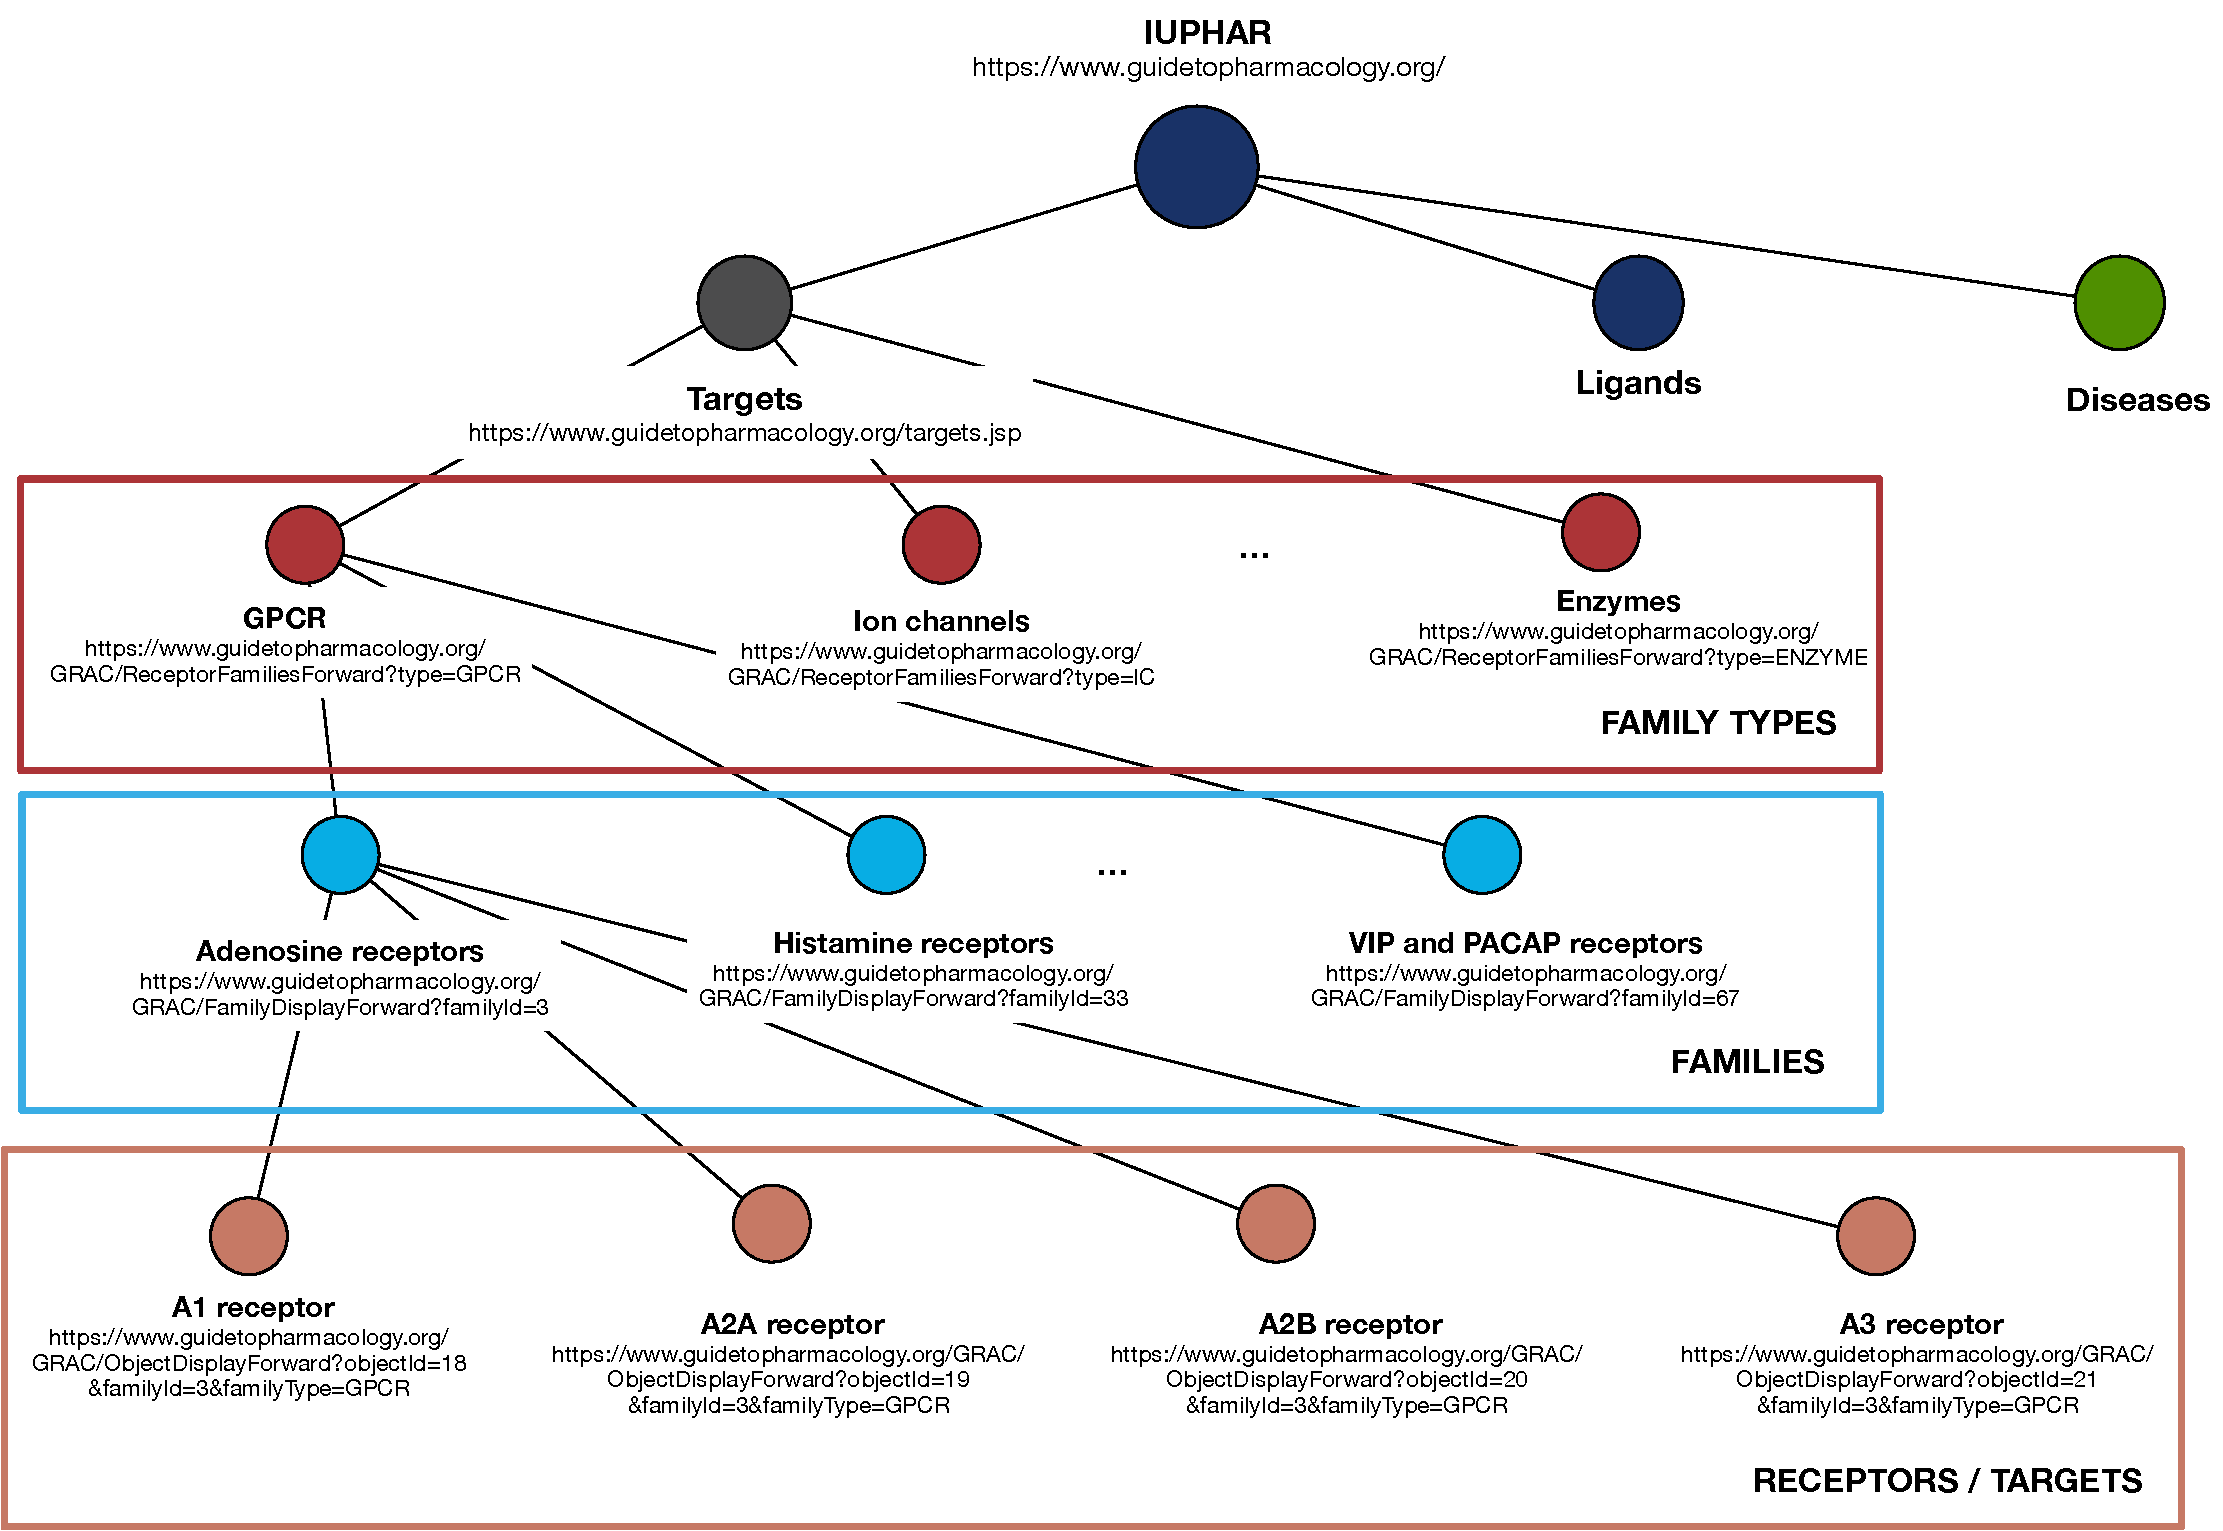
\includegraphics[width=.9\textwidth]{figures/iuphar_schema}
  \caption{Partial map of the GtoPdb hierarchical structure grouping the targets into families and family types.}
  \label{figure:iuphar_schema}
\end{figure}

As use case we refer to the IUPHAR/BPS Guide to Pharmacology \citep{iuphar2018} or  GtoPdb\footnote{\url{https://www.guidetopharmacology.org/}}.
GtoPdb is a well-known and well structured scientific relational database that contains expertly curated information about diseases, drugs in clinical use, their cellular targets, and the mechanisms of action on the human body. 
It is curated and maintained by the GtoPdb Committee, and by 96 subcommittees, comprising 512 scientists collaborating with in-house curators that draw the information contained in the database from high-quality pharmacological and medicinal chemistry literature.
Circa 1000 researchers from many parts of the world have contributed to the database. The curators desire to give recognition to the contributors that led to some early work on data citation~\citep{buneman2006cite}.  

GtoPdb is relational, but its logical structure is hierarchical, as shown in Figure \ref{figure:iuphar_schema}, and the information contained in the database is also organized into webpages focused on specific diseases, targets or ligands and families (i.e., groups) of them for easier access by the users. 
As depicted in Figure \ref{figure:iuphar_schema}, the database can be thought of as a tree where the root is the database itself in its entirety; the first level is composed of the Targets, Ligands, and Diseases considered in their entirety. 
In this paper, we focus on target and target families; thus, in the figure, at the third level, we show some of the family types, that is, groups of targets. At the third level, we show families of targets, a finer level of granularity, and finally, at the last level, the single targets, also known as receptors. 

\begin{figure}[]
\centering
  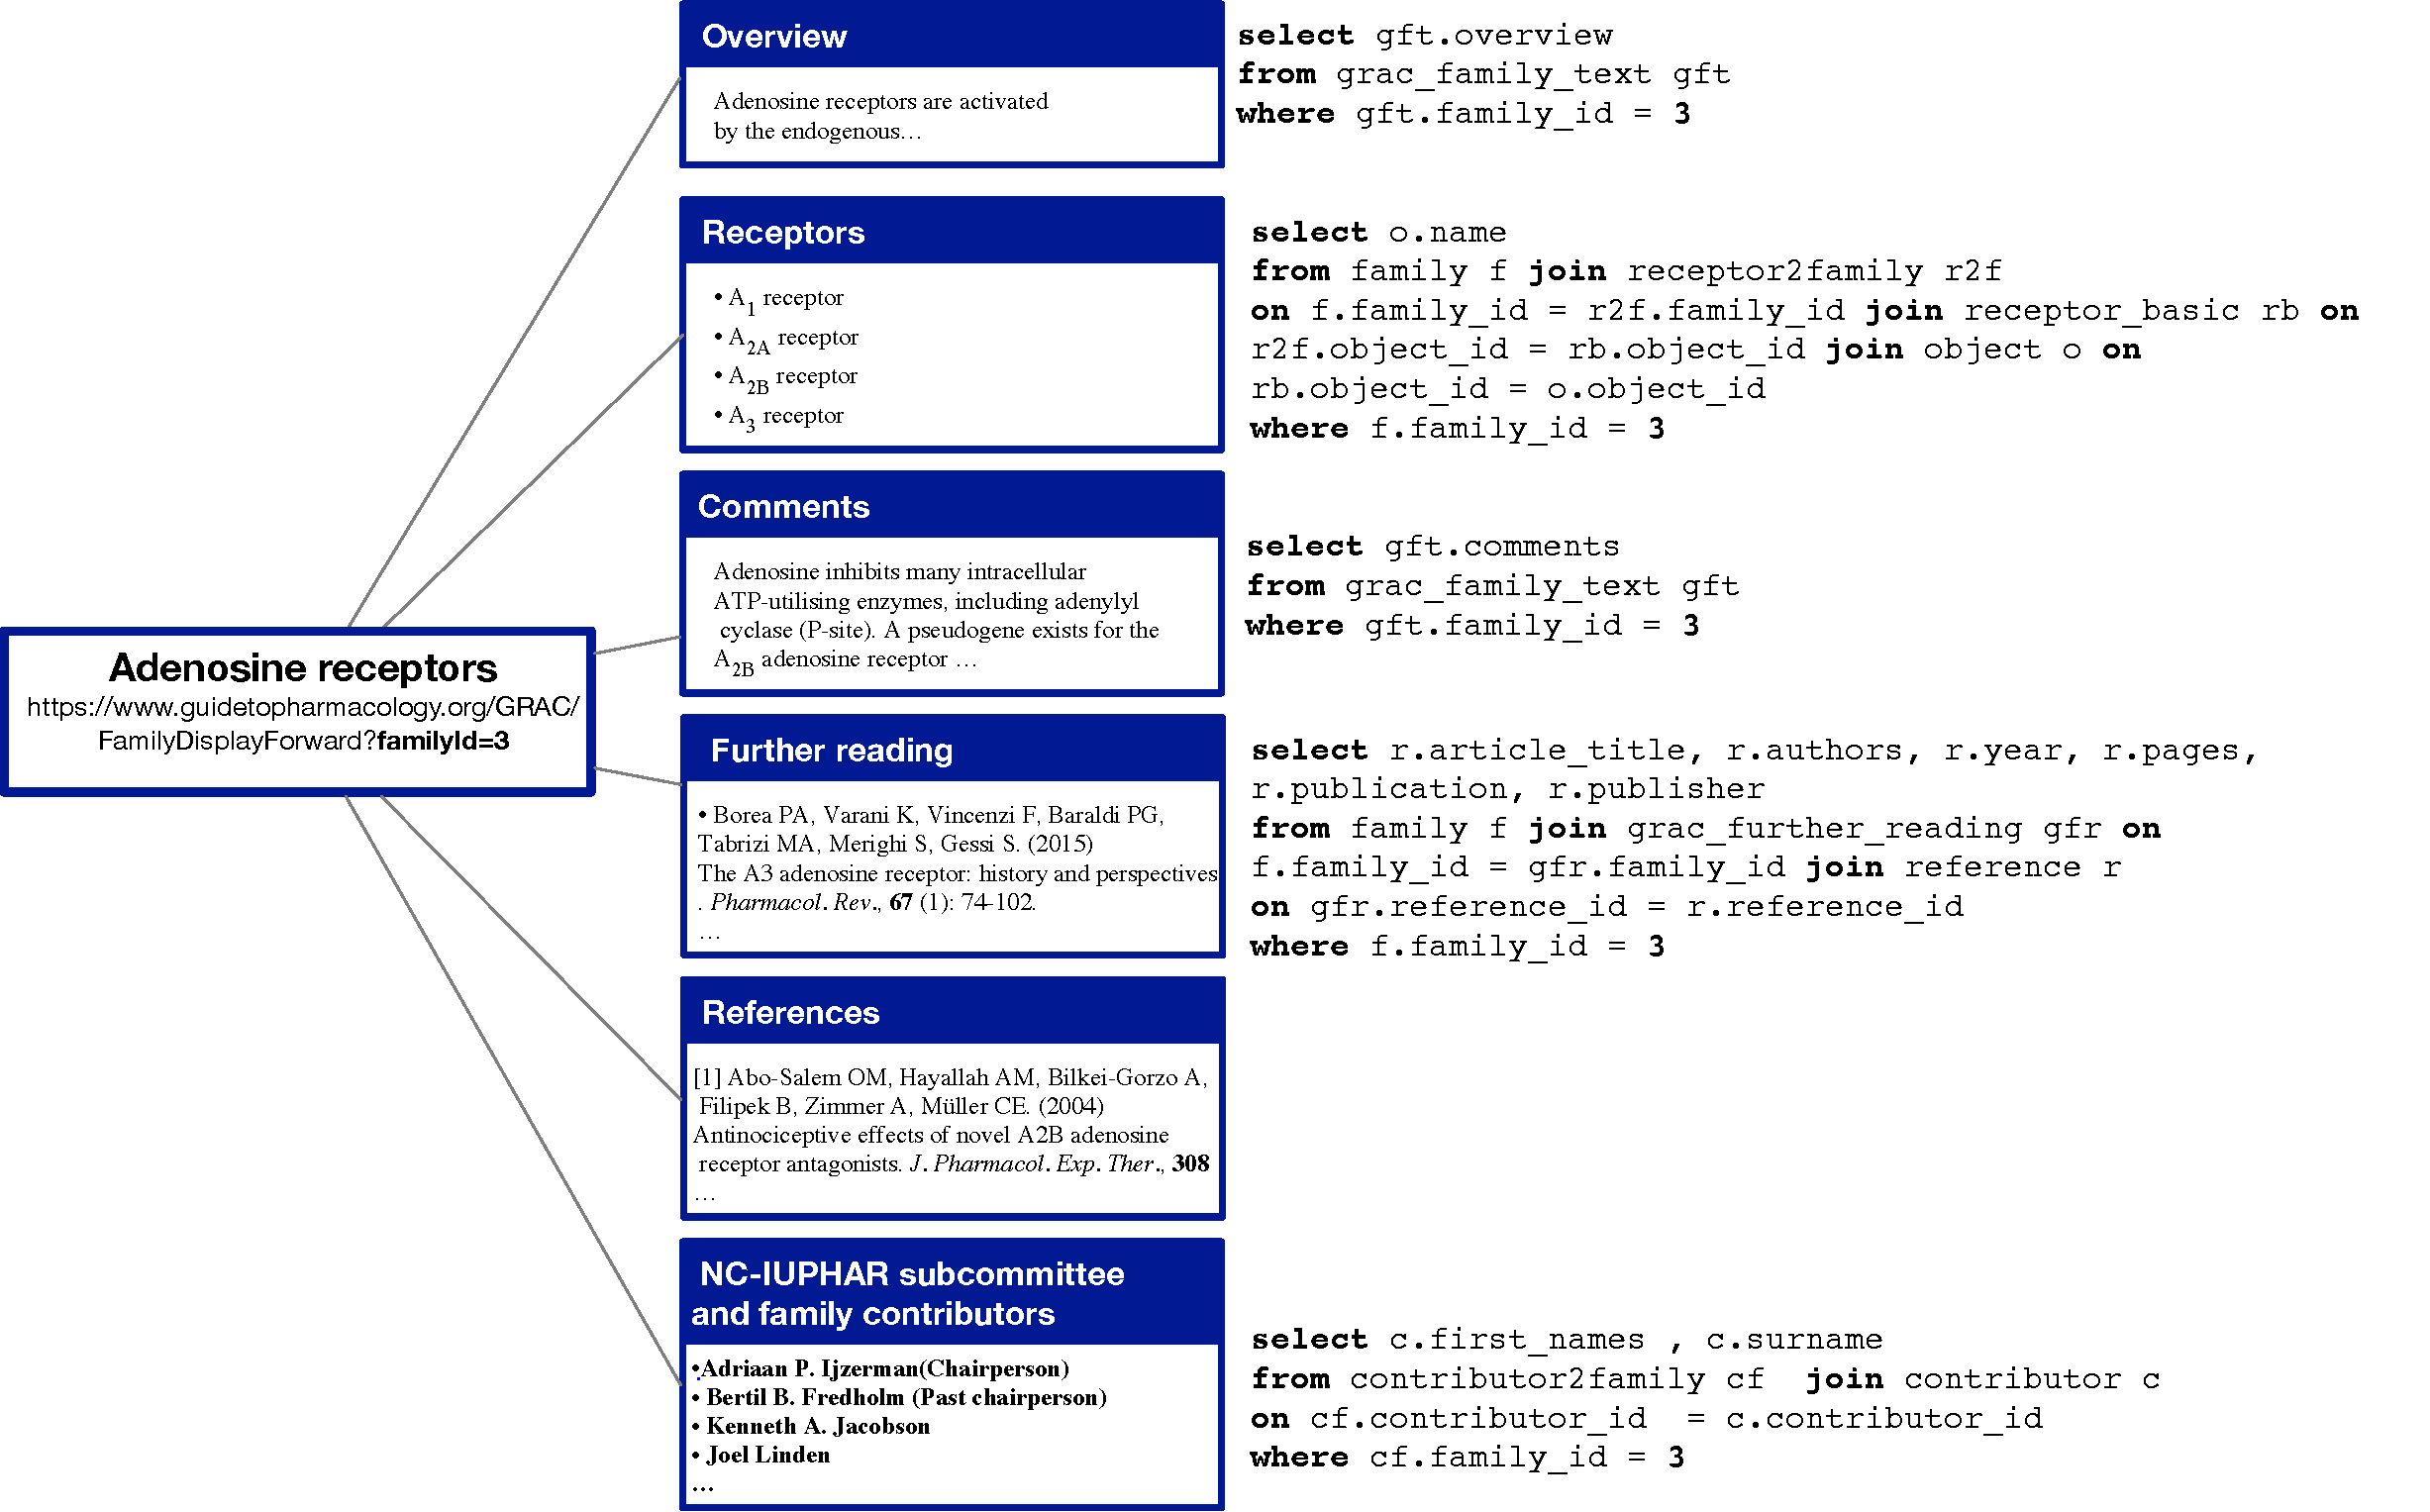
\includegraphics[width=1\textwidth]{figures/family_structure}
  \caption{Basic web-page structure of ``Adenosine receptors'' family (ID 3), with queries used to retrieve the information contained in every section, except references.}
  \label{figure:family_structure}
\end{figure}


The GtoPdb provides access to the webpages corresponding to all these nodes through URLs, as shown in the figure. 
The webpages corresponding to target families all present a similar structure, as shown in Figure \ref{figure:family_structure} for the ``Adenosine receptors'' family. 
Each page has an \emph{Overview}, a brief text describing the content of the page; a list of \emph{Receptors} composing the family; a section of \emph{comments} about the family;
the \emph{References}, a list of the papers consulted by the curators of the page, similar to a reference list of a paper;
the \emph{further reading} list, reporting papers that an interested reader may want to consult to obtain more insight on the family; and a final section called \emph{How to cite this family page}, containing text snippets useful to cite the specific page or the whole database. 
In Figure \ref{figure:family_structure}, we show the SQL code that retrieves the information that is used to build the corresponding sections (apart from the References section).
Therefore, each family page can be considered a full-fledged traditional publication, comprising title, authors, abstract (the overview), content, and references. 

What happens is that many papers in the literature use the GtoPdb's information without including a reference to the specific page being cited. 
Instead, they only cite one data paper describing GtoPdb (e.g., the more recent \citep{iuphar2018}) and refer to targets, ligands, diseases, etc. only by their name. 
Thus, the citations to the specific families turn out to be \emph{de-facto} ``hidden'' to the citation systems such as Google Scholar, and useless for the computation of bibliometrics. 

In specific ``lucky'' circumstances, as in the case of papers available in PDF and published in the British Journal of Clinical Pharmacology~\footnote{\url{https://bpspubs.onlinelibrary.wiley.com/journal/13652125}} (BJCP), when a  family, a ligand, a receptor name, etc. are used, they also have a hyperlink pointing to the corresponding webpage in GtoPdb. Therefore, the citations to the families can be spotted and counted using the URLs reported in the papers.
These citations to GtoPdb webpages, in any case, are not counted as such by the citation systems, so they are not converted into credit for curators and collaborators. 

For our running example, consider Table \ref{table:running_example}. This simplified version of GtoPdb illustrates three relations: \texttt{family}, \texttt{contributor} and \texttt{contributor2family}.

The first table's tuples represent four families, composed of three attributes: the id of the family, its name, and type. 
\texttt{contributor} contains the people who have helped to generate the data of the database.
Finally, table \texttt{contributor2family} serves as a link between the families and the people who contributed to them.
For instance, ``John Smith'' ($\mathtt{c_1}$) contributed to ``Dopamine Receptors'' ($\mathtt{f_1}$) as well as to the ``YANK Family'' ($\mathtt{f_4}$). We use this example throughout the rest of the paper.

\begin{table*}[]
\centering
\begin{tabular}{| l | cc |}
\multicolumn{3}{c}{\textbf{family}}\\
\hline
 id & name & type \\
  \hline
  $f_1$ & Dopamine Receptors & gpcr \\
  $f_2$ & Bile Acid Receptor & gpcr \\
  $f_3$ & FAK Family         & enzyme \\
  $f_4$ & YANK Family        & enzyme \\
\hline
\end{tabular}	
\begin{tabular}{| l |c c|}
\multicolumn{3}{c}{\textbf{contributor2family}}\\
\hline
 id & family\_id & contributor\_id \\
  \hline
  $c2f_1$ & $f_1$ & $c_1$ \\
  $c2f_2$ & $f_1$ & $c_2$ \\
  $c2f_3$ & $f_2$ & $c_3$ \\
  $c2f_4$ & $f_4$ & $c_1$ \\
\hline
\end{tabular}		
\begin{tabular}{| l |c c|}
\multicolumn{3}{c}{\textbf{contributor}}\\
\hline
 id & Name & Country \\
  \hline
  $c_1$ & John Smith & UK \\
  $c_2$ & Jim Doe & UK \\
  $c_3$ & Hans Zimmerman & Germany \\
  $c_4$ & Roberta Rossi & Italy \\
\hline
\end{tabular}		
\caption{Example of a database composed by three tables. \texttt{family} includes some receptor families in the database; \texttt{contributor}, with the name and country of contributors of the database; \texttt{contributor2family}, connecting the contributors to the families they contributed to.}
\label{table:running_example}
\end{table*}
